%!TEX root = tcc_final.tex
\chapter{Desenvolvimento}\label{chap4:desenvolvimento}

\frm[inline]{Digamos que isto está um pouco, curto. }
    % - Falar sobre as informações necessárias para o desenvolvimento
    % - Falar sobre o local onde o CPA foi integrado (em detalhes)
    % - Falar sobre o desenvolvimento em si
    %   - Colocar fórmulas dos vetores
    %   - Explicar profundamente as equações
    % - Falar sobre o que foi feito para a coleta dos resultados
    %   - Criação dos tópicos para publicar t_cpa e d_cpa
    
    %O desenvolvimento deste trabalho resume-se à implementação da Equação~\ref{eq:tcpa} e da Equação~\ref{eq:dcpa}.\frm{Se eu bem me recordo, tu tiveste que mexer em bem mais coisas para fazer tudo rodar, não? Eu diria que esta frase vende teu trabalho barato... Tenta explicar que tu tiveste que tunar parâmetros também...} 
    %Obtendo os valores resultantes, aplica-se a Desigualdade~\ref{eq:cpaThreshold} para determinar se há risco de colisão ou não. Para tal, usou-se informações referente à posições e velocidades das embarcações que já estavam disponíveis no sistema base. Além disso foi preciso identificar onde, no sistema desenvolvido por Jurak~\cite{Jurak2020COLREGS}, a implementação do ponto de maior proximidade (do inglês \textit{"Closest Point of Approach"} - CPA) seria realizada, para que implementação e integração ocorressem paralelamente. 
    %Como citado no Capítulo~\ref{subchap3:sistema_base}, o sistema base cria obstáculos artificiais para fazer com que seu planejador local encontre uma rota que seja compatível com as COLREGS. 
    %Logo, identificamos que os obstáculos virtuais deveriam ser criados somente quando houver risco de colisão, caso contrário os obstáculos virtuais não devem ser criados. 
    %A Figura~\ref{fig:chap4_fluxograma_inicial} apresenta o fluxograma da rotina onde os obstáculos virtuais são criados antes da implementação do CPA. 
    %Com base no fluxograma apresentado, chegamos a conclusão que a implementação do CPA deveria ser realizada no momento anterior à criação dos obstáculos virtuais. 
    %A Figura~\ref{fig:chap4_fluxograma_final} apresenta o fluxograma da rotina onde os obstáculos virtuais são criados após a implementação do CPA. 
    %Para fins de análise, foi adicionado no sistema base dois tópicos para a publicação do \tcpa e do \dcpa encontrados. Essas informações foram coletadas dos tópicos criados durante as execuções dos testes e gravadas em um arquivo \textit{".bag"}. As informações coletadas serão apresentadas no Capítulo~\ref{chap5:resultados}.
    
    
    
    Dado que o objetivo deste trabalho é capacitar o sistema base a avaliar as posições futuras das embarcações envolvidas em um encontro para identificar um risco de colisão, nossa implementação se dará no mecanismo de comportamento reativo do sistema base. Como explicado anteriormente, o comportamento reativo de um sistema para veículos de superfície não tripulados (do inglês \textit{"Unmanned Surface Vehicle"} - USV) é responsabilidade do planejador local~\cite{Jurak2020COLREGS}. Com isso, reapresentamos a arquitetura do sistema baes na Figura~\ref{fig:chap4_onde_implementar_cpa} indicando onde realizaremos a implementação do CPA.
    
    
    \begin{figure}
        \centering
        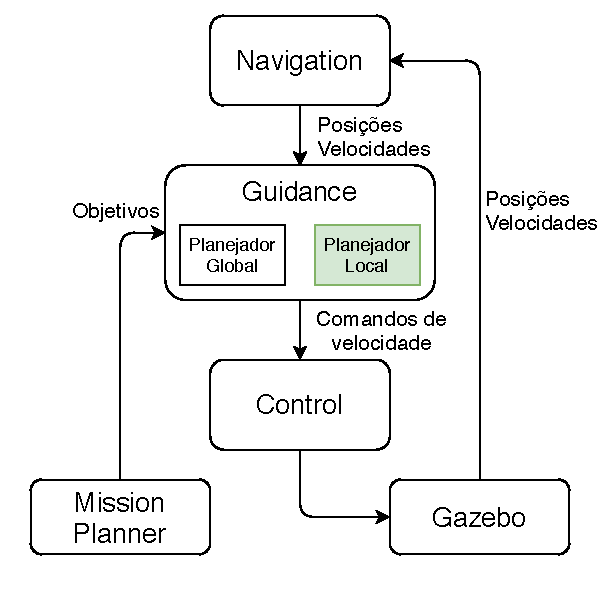
\includegraphics{fig/chap4/onde_implementar_cpa.pdf}
        \caption{Indicação na arquitetura base de onde será realizada a implementação}
        \label{fig:chap4_onde_implementar_cpa}
    \end{figure}
    
    Sempre que houver uma embarcação nas proximidades do USV, o sistema base cria obstáculos artificiais no mapa de custo do planejador local para induzi-lo a realizar uma manobra de evasão em conformidade com as regulamentações de prevenção de colisões no mar (do inglês \textit{"COLision REGulations at Sea" - COLREGS}. Como o ponto de maior proximidade (do inglês \textit{"Closest Point of Approach"} - CPA) 
    é um método para mensurar o índice do risco de colisão (do inglês \textit{"Collision Risk Index"} - CRI), concluímos que o CPA deveria ser avaliado antes de realizar a criação dos obstáculos virtuais, pois se não há risco de colisão os obstáculos virtuais não devem ser criados.
    
    O fluxograma inicial (antes de implementação do CPA) da rotina que realiza a criação dos obstáculos virtuais é apresentado pela Figura~\ref{fig:chap4_fluxograma_inicial}. Inicialmente, é verificado a validade do objetivo recebido do nodo \textit{"mission planner"}. Se o objetivo atual e o objetivo anterior a este forem inválidos, o sistema não fará nada. Porém, se o objetivo atual for inválido mas o anterior a este for válido, o sistema deverá utilizar o último comando de velocidade gerado. 
    Já se o objetivo atual for válido e não houver nenhuma embarcação nos arredores do USV, o sistema planejará a rota local e gerará os comandos de velocidade. Contudo, se o objetivo atual for válido e houver uma embarcação nas proximidades do USV, o sistema criará obstáculos virtuais no mapa de custo do planejador local, planejará a rota possível e então gerará os comandos de velocidade.
    
    \begin{figure}
        \centering
        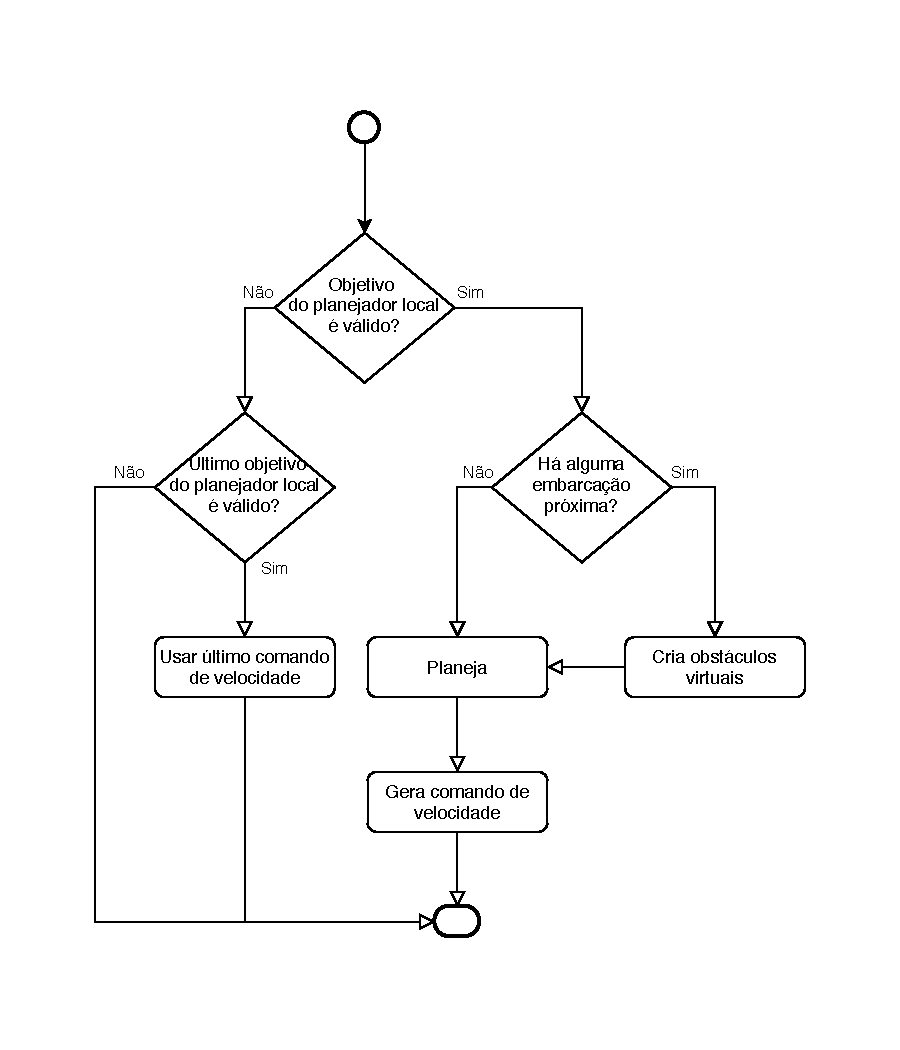
\includegraphics{fig/chap4/find_best_path_diagram_no_cpa.pdf}
        \caption{Fluxograma inicial da rotina onde o CPA foi adicionado.}
        \label{fig:chap4_fluxograma_inicial}
    \end{figure}
    
    A implementação do CPA fez uso das informações de posição e velocidade das embarcações envolvidas no encontro. Essas informações já eram utilizadas na rotina que cria os obstáculos virtuais, sendo necessário apenas transmitir essas informações através de parâmetros para a rotina que realizará o cálculo do CPA. 
    
    
    \begin{figure}
        \centering
        \includegraphics{}
        \caption{Caption}
        \label{fig:my_label}
    \end{figure}
    
    \begin{figure}
        \centering
        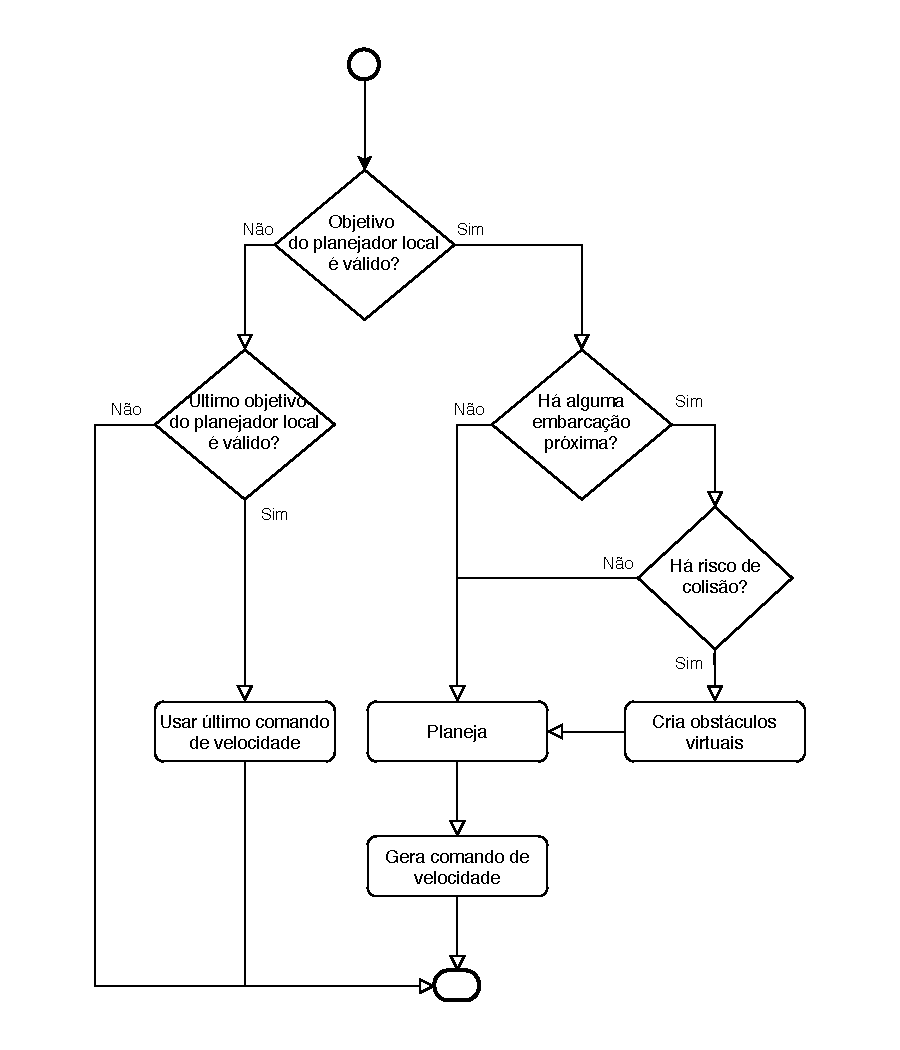
\includegraphics{fig/chap4/find_best_path_diagram_cpa.pdf}
        \caption{Fluxograma final da rotina onde o CPA foi adicionado.}
        \label{fig:chap4_fluxograma_final}
    \end{figure}
    
    % --------------------------------------
    % -------------- QUESTÕES --------------
    % --------------------------------------
    
    % 1) Explicação do CPA deveria estar, na verdade, no capítulo de fundamentação teórica
    % 2) Penso em colocar código no documento final, sinto que não há muito o que falar da implementação, apenas que implementamos os cálculos.